\chapter{Динамические машины состояний}
\label{appendix:fsm-machine-prog}

\begin{figure}
    \centering
    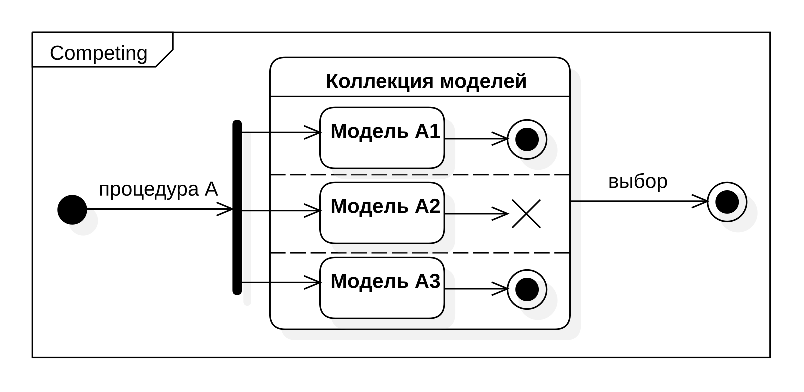
\includegraphics[width=0.65\linewidth]{images/umff-competing-diagram-02.eps}
    \caption{Пример машины конечных состояний порождаемой
    элементом обобщённого поведения <<competing>>}
    \label{fig:competing-example}
\end{figure}

\begin{figure}
    \centering
    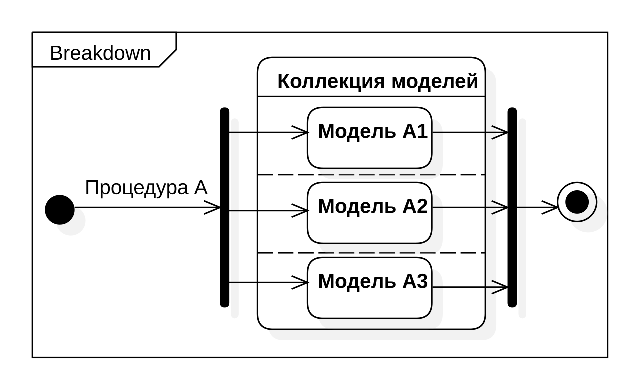
\includegraphics[width=0.55\linewidth]{images/umff-breakdown-diagram-01.eps}
    \caption{Пример машины конечных состояний порождаемой
    элементом обобщённого поведения <<breakdown>>}
    \label{fig:breakdown-example}
\end{figure}

\begin{figure}
    \centering
    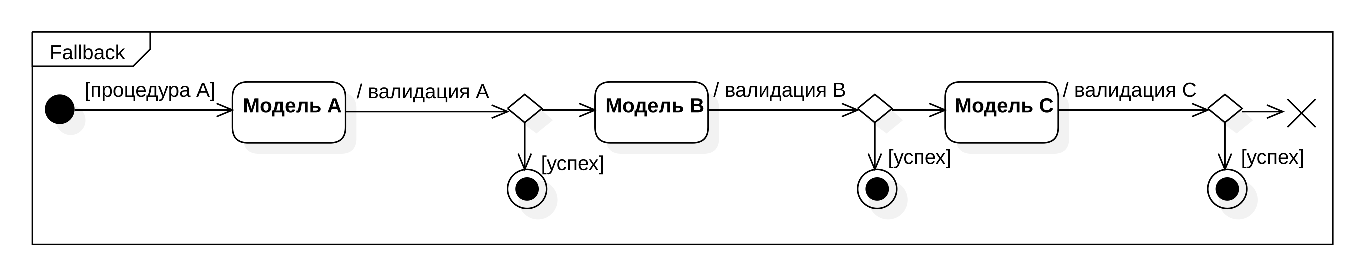
\includegraphics[width=0.95\linewidth]{images/umff-fallback-example-01.eps}
    \caption{Пример машины конечных состояний порождаемой элементом обобщённого
    поведения <<fallback>>}
    \label{fig:fallback-example}
\end{figure}


\begin{figure}
    \centering
    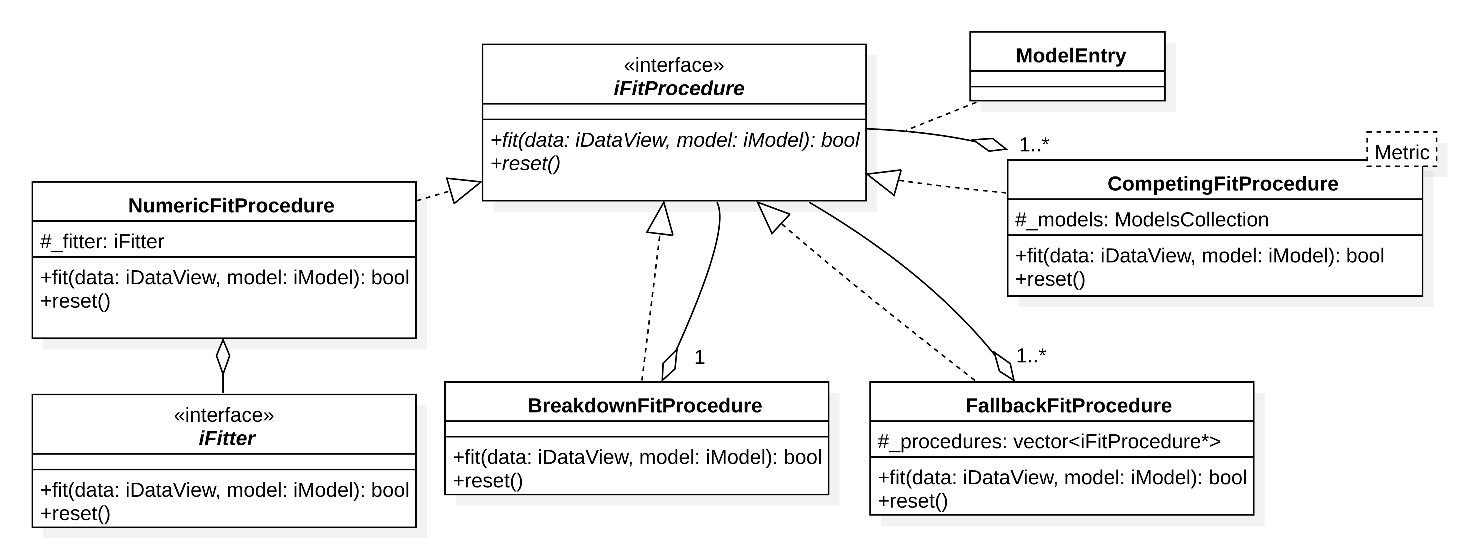
\includegraphics[width=1\linewidth]{images/BasicFitProcedcureDiagram-01.eps}
    \caption{Диаграмма классов элементов обобщённого поведения}
    \label{fig:umff-basic-fitting-procedures}
\end{figure}

В качестве программной реализации, рассмотрим декомпозицию на классы показанную
на Рисунке~\ref{fig:umff-basic-fitting-procedures}. Интерфейс \texttt{iFitProcedure}
фиксирует наиболее общий контракт варианта использования процедуры через
объявление сигнатур методов \texttt{fit()} и \texttt{reset()}, соответствующих
общим для всех процедур этапам жизненного цикла.

В частности, простейший вариант использования выражается
реализацией~\texttt{NumericFitProcedure}, делегирующей выполнение конкретным
численным процедурам через интерфейс \texttt{iFitter}.

Вариант использования с декомпозицией модели реализован в классе
\texttt{BreakdownFitProcedure}, в агрегирующим единственную подчинённую
процедуру через её полиморфную базу.

Вариант использования с выбором подходящей модели реализован в
классе~\texttt{FallbackFitProcedure} и агрегирует упорядоченный набор
экземпляров подклассов~\texttt{iFitProcedure}.

Вариант использования с выбором наилучшего результата должен быть
параметризован метрикой по которой определяется наилучшее соответствие.
Поскольку на данном уровне общности отсутствует требование конкретной
топологии данных, а вычисление метрики ожидается довольно частым,
был выбран статический полиморфизм. Реализация предложенная в шаблонном
классе \texttt{CompetingFitProcedure} параметризуется типом метрики.
В то же время, чтобы сохранить гибкость в стратегии
принятия решений, и предоставить пользовательскому коду возможность
определять подклассы, реализующие, например, ленивое вычисление,
коллекция моделей строится через посреднический тип, содержащий
дополнительные аннотации к экземплярам моделей (например, значение
метрики).

\begin{figure}
    \centering
    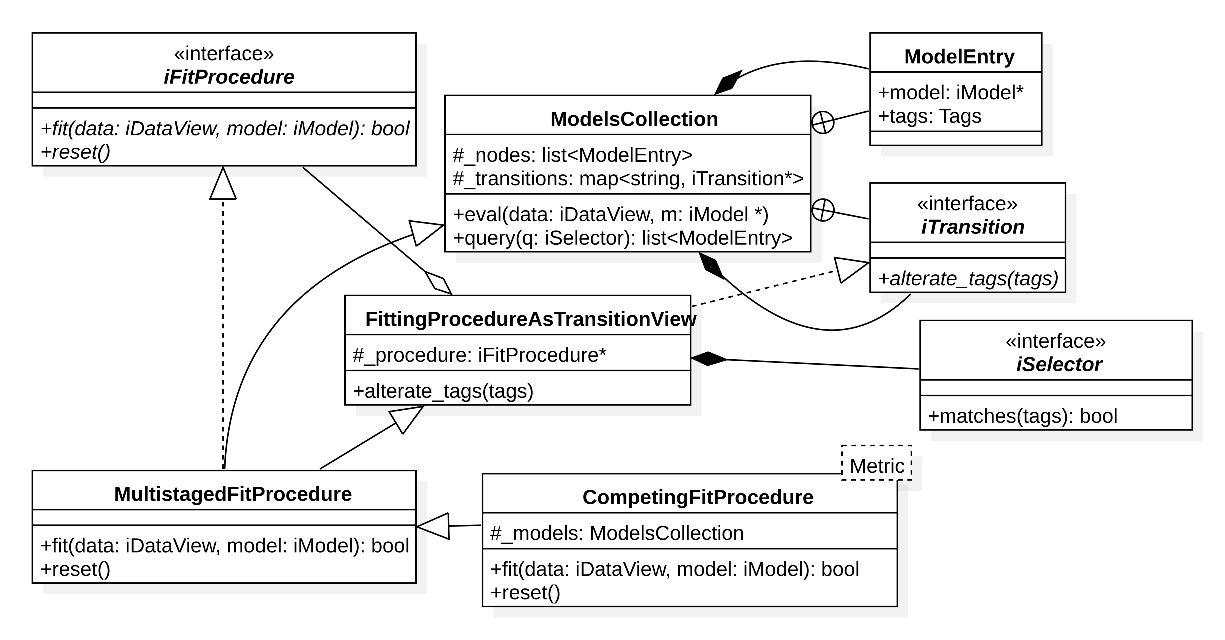
\includegraphics[width=1\linewidth]{images/umff-CompetingFitProcedureClassDiagram-01.eps}
    \caption{Диаграмма классов иллюстрирующая объектную
    модель~\texttt{ModelsCollection}}
    \label{fig:CompetingFitProcedureCollection}
\end{figure}

Более подробно реализация \texttt{CompetingFitProcedure} показана
на Рисунке \ref{fig:CompetingFitProcedureCollection}.  Реализация
опирается на класс \texttt{ModelsCollection},
управляющий порождаемой машиной конечных состояний над множеством состояний
модели~$m_i$ дополненных набором текстовых меток~$t_i$, согласно
правилам перехода~$\{T_j\}$. Каждый
элемент множества~$T_j$ задаёт правило перехода,
дополняя процедуру~$P_k$ правилом альтерации~$t_j = A_j(t_i)$
и предикатом текстовых меток~$C_j(t_i)$, что
символически отразим как $T_j:=\{P_k, A_j, C_j\}$. Выполнению процедуры
$P_j(m_i) = m_j$ в таком расширенном контексте соответствует
операция $T_j:C_j(t_i);~T_j(\{m_i,t_i\}) = \{P_j(m_i), A_j(t_i)\} = \{m_j, t_j\}$.
Иными словами, аннотирование модели текстовыми метками нужно затем
чтобы на данном уровне общности снабдить абстрактную модель логическими
предикатами для выбора соответствующего перехода. Экземпляры
множества~$\{m_i,t_i\}$ соответствуют типу
данных \texttt{ModelsCollection::ModelEntry}, а правилам
перехода~$T_j=\{P_j, A_j, P_j\}$ отвечает интерфейс~\texttt{ModelsCollection::iTransition}.

%С точки зрения модели данных класс \texttt{ModelsCollection} содержит:
%\begin{itemize}
%    \item Атрибут \texttt{_nodes} --- набор состояний
%    модели ${m_i,t_i}$, организованный в виде связного графа,
%    соответствующей машине конечных состояний. В узлах машины представляемых
%    структурой \texttt{ModelEntry}, помимо ассоциированного
%    экземпляра модели, содержится набор текстовых
%    меток~\texttt{tags}.
%    \item Набор переходов заданных экземплярами
%    подклассов~\texttt{iTransition} в форме ассоциативного
%    массива.  Экземпляры подклассов~\texttt{iTransition} определяют
%    логический предикат перехода посредством реализации~\texttt{iSelector},
%    и реализуют метод~\texttt{alterate_tags()}
%    изменяющий набор текстовых меток модели в новом состоянии.
%\end{itemize}

Метод \texttt{eval()} класса~\texttt{ModelsCollection}
принимает на вход экземпляр модели~$m_0$, набор данных~$x$,
и реализует следующий рекурсивный алгоритм прохода в глубину
со стеком:
\begin{enumerate}
    \item Создаётся новый экземпляр структуры \texttt{ModelEntry}
    ${m_i,\vec{t}_i} = \{m_0, \vec{t}_0\}$, инициализированный
    исходной моделью и набором начальных текстовых меток, заданных
    для экземпляра \texttt{ModelsCollection}.
    \item Среди множества правил перехода выбирается первый
    элемент $T_j$ со связанным предикатом, отвечающий $t_i$. Если
    таковой найден, выполняется
    переход~$T_j:C_j(t_i);~T_j(\{m_i,t_i\}) = \{m_j, t_j\}$, новое
    состояние сохраняется в стеке (\emph{stack push}), и для $\{m_j,t_j\}$
    повторяется алгоритм с п.2.
    \item Если перехода с соответствующим предикатом не
    найдено~($T_j:C_j(\{m_i,t_i\})\rightarrow\varnothing$) и
    стек не пуст то состояние изымается из стека (\emph{stack pull}),
    алгоритм повторяется с п.2. с прежним состоянием.
    \item Если $T_j:C_j(\{m_i,t_i\})\rightarrow\varnothing$ и
    стек пуст, алгоритм завершён.
\end{enumerate}

Вспомогательный метод~\texttt{query()} класса~\texttt{ModelsCollection}
параметризуется предикатом $C(t)$ и осуществляет выбор $\{m_i,t_i\}:C(t_i)$.

Промежуточный класс~\texttt{MultistagedFitProcedure} реализует
интерфейс~\texttt{iFitProcedure} посредством делегирования выполнения
соответствующим методам~\texttt{ModelsCollection}. При этом,
результат применения процедуры (\texttt{MultistagedFitProcedure::fit()})
выраженной в~\texttt{ModelsCollection} является первый результат в
списке возвращённом запросом~\texttt{ModelsCollection::query()},
согласно предикату параметризующему экземпляр~\texttt{MultistagedFitProcedure}.
Это поведение изменено в шаблонном
классе~\texttt{CompetingFitProcedure<Metric>}, который осуществляет
отбор результатов \texttt{query()} посредством параметра-метрики,
таким образом реализуя вариант
использования~<<\emph{выбор наилучшего результата}>>.

Заметим, что описанная реализация процедур имеет дело с максимально
общим описанием моделей и данных. За исключением элемента обобщённого
поведения осуществляющего декомпозицию~(\emph{breakdown}), для модели фиксируется
только следующее поведение:
\begin{itemize}
    \item Вычисление модели на данных идемпотентно (т.е. это \emph{чистая функция},
    зависящая только от $\{x, p\}$).
    \item Модель рефлексивна (т.е. допускает копирование посредством
    интерфейса \texttt{iModel}).
\end{itemize}

Требование накладываемое декомпозицией существенно более строго и
вводит в рассмотрение транзитивное отношение включения
множеств моделей: $m_1 \in m_2, ~m_2 \in m_3 \implies m_1 \in m_3$. Этот вариант
использования очень важен с практической стороны, поскольку большинство
рассмотренных задач физической реконструкции так или иначе имеют
дело с моделями допускающими декомпозицию, в том числе с неоднозначностями,
и при этом принятие решений (выбор варианта) должно производиться на основе
дополнительной информации предоставляемой алгоритмами аппроксимации.
Например, на разных стадиях анализа алгоритм фитирования трека должен
опираться не только на~$\chi^2$ трека, но и учитывать количество сработавших
детекторов, -- до окончания процедуры физического выравнивания,
выбор наиболее длинного трека более предпочтителен чем выбор наиболее
правдоподобной оценки.

\begin{figure}
    \centering
    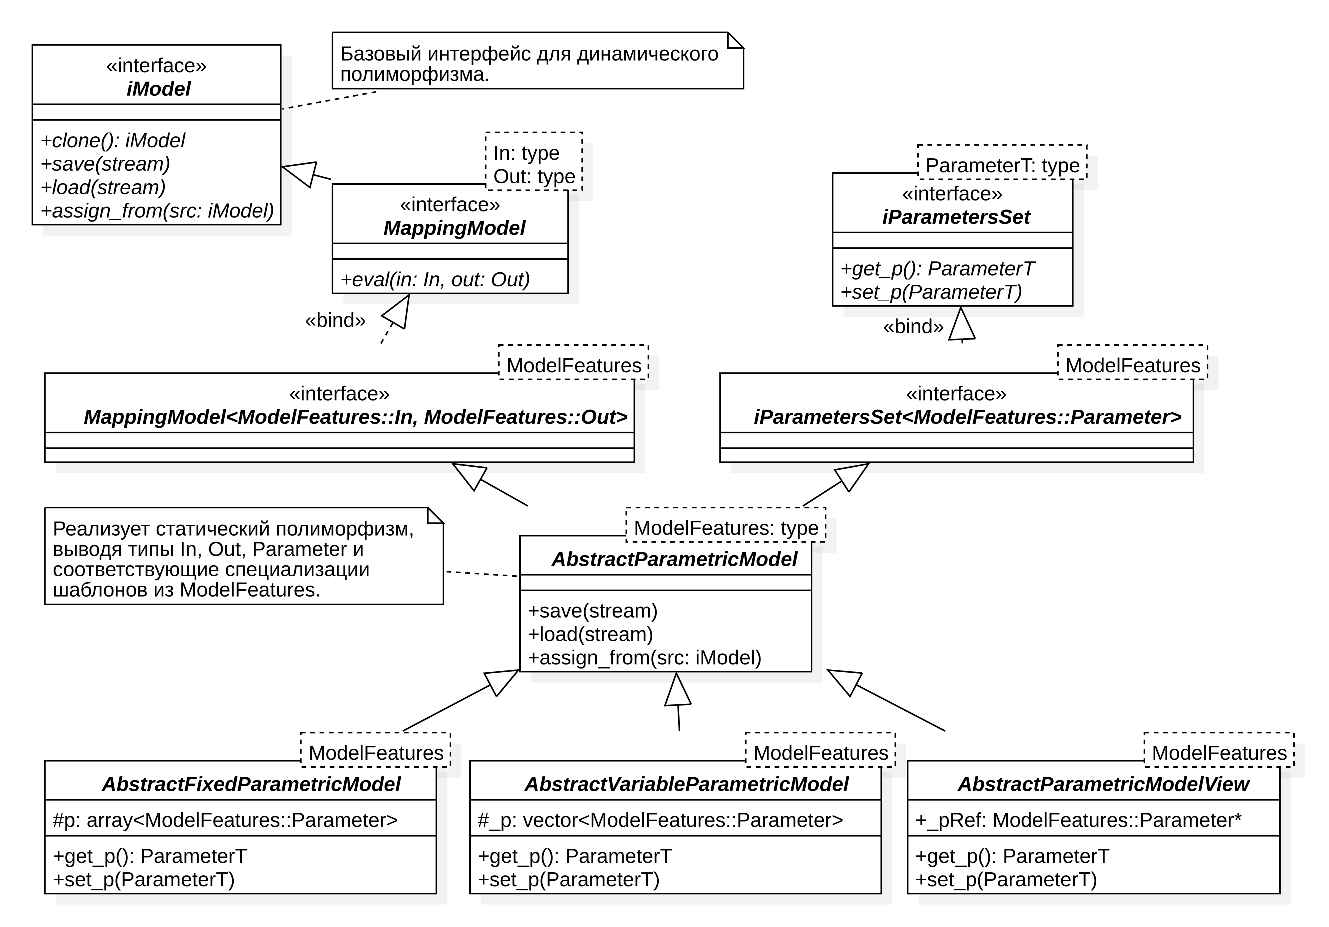
\includegraphics[width=1\linewidth]{images/umff-BasicModelClassDiagram-01.eps}
    \caption{Диаграмма классов показывающая типовые реализации интерфейса \texttt{iModel}}
    \label{fig:basic-model-classes}
\end{figure}

Рассмотрим систему классов на Рисунке \ref{fig:basic-model-classes}. Упоминавшийся ранее
интерфейс \texttt{iModel} задаёт абстрактную базу удовлетворяющую наиболее общим
требованиям сценариев представленных элементами <<\emph{fallback}>>
и <<\emph{competing}>>. В предположении о том, что набор параметров~$\vec{p}$
гомогенен (представим в виде массива значений одного и того же типа),
этот интерфейс может быть сведён средствами статического
полиморфизма до абстрактной реализации~\texttt{AbstractParametricModel}.

Дополнительные предположения о типе ассоциации определяют реализацию интерфейса
доступа к значениям параметров.

Статическая композиция частично реализованная в абстрактном базовом
классе~\texttt{AbstractFixedParametricModel<>} нужна для моделей с
фиксированным числом параметров -- например, аппроксимация
одиночной $N$-параметрической функцией отдельного пика, линейной модели
движения частицы, отдельного ливневого профиля и т.д.

Динамическая композиция частично реализованная в абстрактном
классе~\texttt{AbstractVariableParametricModel<>} нужна для моделей с
переменным числом параметров. Такие модели используют различные алгоритмы
поиска, задания начальных условий, а также алгоритмы апостериорной
коррекции (например, удаления вырожденных членов после аппроксимации).

Агрегация параметров декомпозированной модели реализуется через абстрактный
класс-прослойку -- \emph{вид}
\texttt{AbstractParametricModelView<>}. Экземпляры этого класса,
всегда ассоциированы с экземпляром подкласса~\texttt{AbstractParametricModel}
и в конечном счёте всегда предоставляют доступ к значениям параметров
содержащихся в композиционном классе, реализуя таким образом отношение
включения множеств.